\subsection{Phase Portraits}
This part of the report shows a total of five different figures with four different regimes, three of the parameter sets were taken from the suggestions in the lab instructions while two were to further illuminate the two-dimensional behaviour of the system at different points in the bifurcation diagram.

For the phase portrait shown in figure \ref{fig:phaseport-2.8}, one can see clear convergence towards a single fixed point.
Due to the removal of a transient period before plotting the evolution, the plot extents are quite small.
Convergence can be seen because the points away from the yellow dot indicating the final convergence of the last evolution are quite dark and therefore need to come from the beginning of a cycle.
Towards the dot there is also a faint brightening of the colour showing that the later iterations end up closer to the convergence point.
\begin{figure}[h]
	\centering
	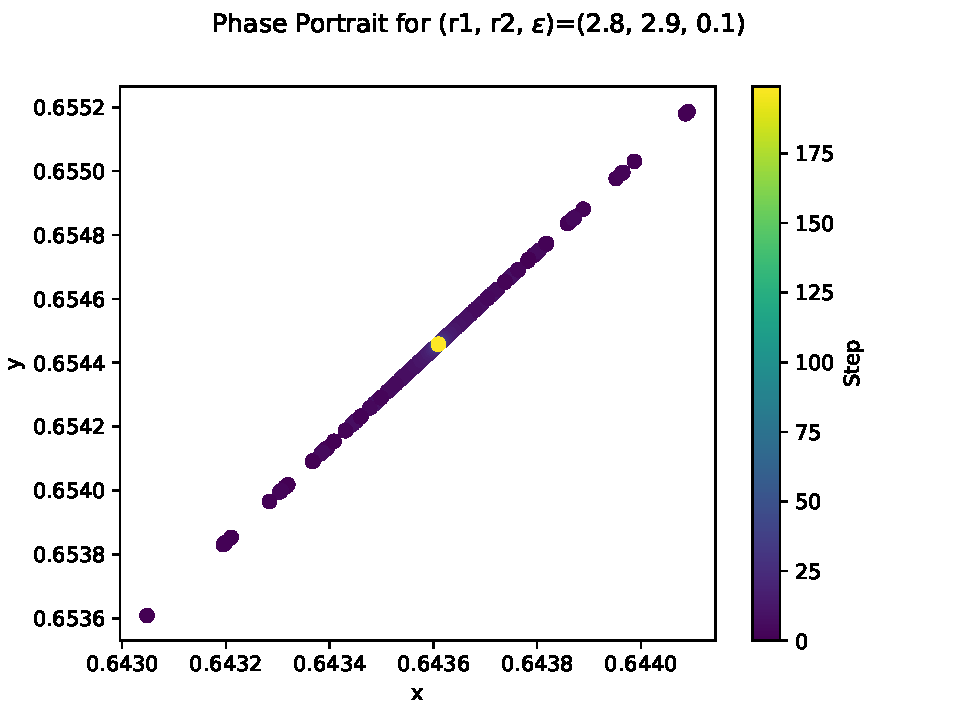
\includegraphics[width=\textwidth]{figs/phase_(2.8, 2.9, 0.1)}
	\caption{Phase Portrait for $\left(r_1, r_2, \epsilon\right) = \left(2.8, 2.9, 0.1\right)$}
	\label{fig:phaseport-2.8}
\end{figure}
\newpage

\begin{figure}[h]
	\centering
	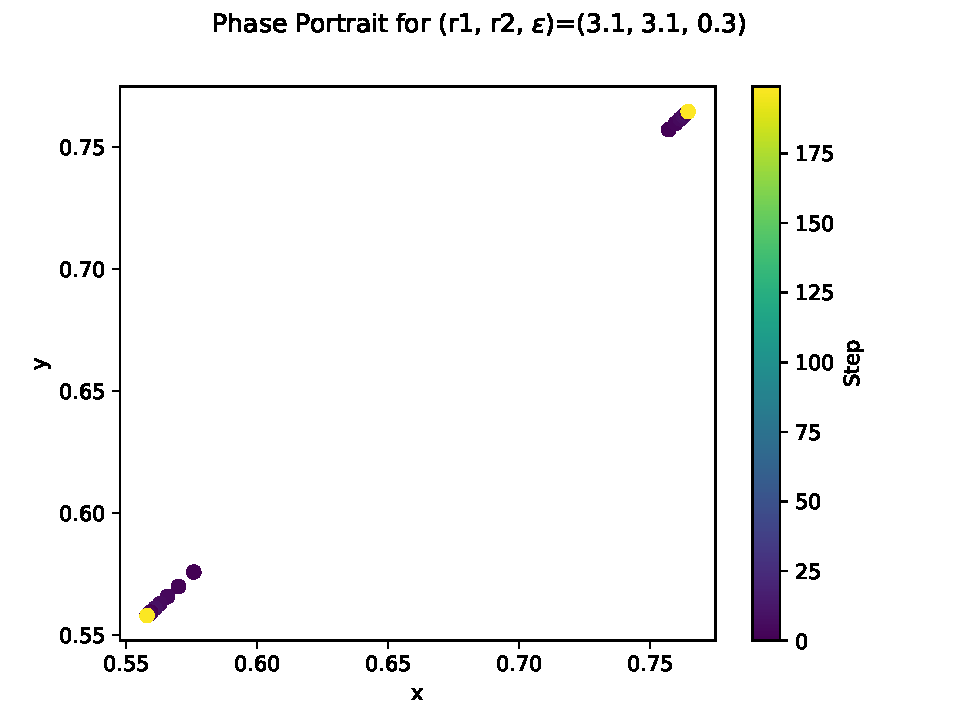
\includegraphics[width=\textwidth]{figs/phase_(3.1, 3.1, 0.3)}
	\caption{Phase Portrait for $\left(r_1, r_2, \epsilon\right) = \left(3.1, 3.1, 0.3\right)$}
	\label{fig:phaseport-3.1-3.1}
\end{figure}
In the next figure, figure \ref{fig:phaseport-3.1-3.1}, we can see the first appearance of a bifurcation in the phase portrait.
This bifurcation means that now two different attractive points exist instead of only one.
As stated in the methods section, a phase portrait like this does not allow to make the distinction between two attractive, fixed points and a period-2 orbit.
As expected from the symmetric case with $r_1 = r_2$, both points lie on the diagonal with $x=y$.
\newpage

\begin{figure}[h!]
\centering
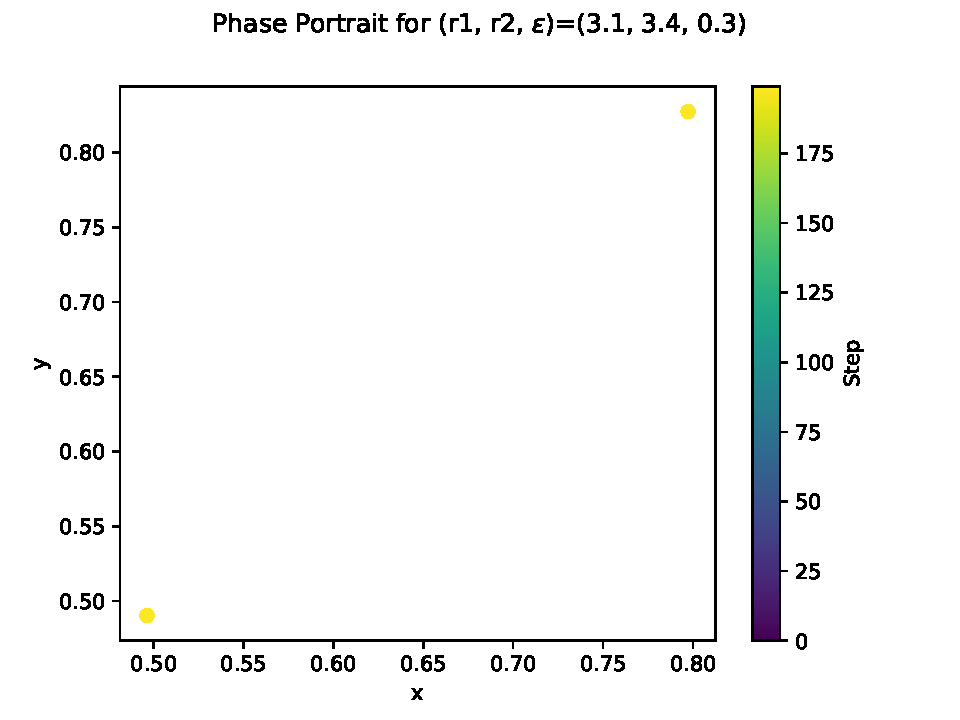
\includegraphics{figs/phase_(3.1, 3.4, 0.3)}
\caption{Phase Portrait for $\left(r_1, r_2, \epsilon\right) = \left(3.1, 3.4, 0.3\right)$}
\label{fig:phaseport-3.1}
\end{figure}
The impact of varying only one parameter can be seen in figure \ref{fig:phaseport-3.1}.
When raising $r_2$ slightly, the bifurcation into two attractive basins remains, while the locations shift.
With this configuration the two points are farther apart and slightly away from the aforementioned diagonal.
Due to the medium strong coupling the displacement is only barely recognizable in the plot.
\clearpage

\begin{figure}[h!]
	\centering
	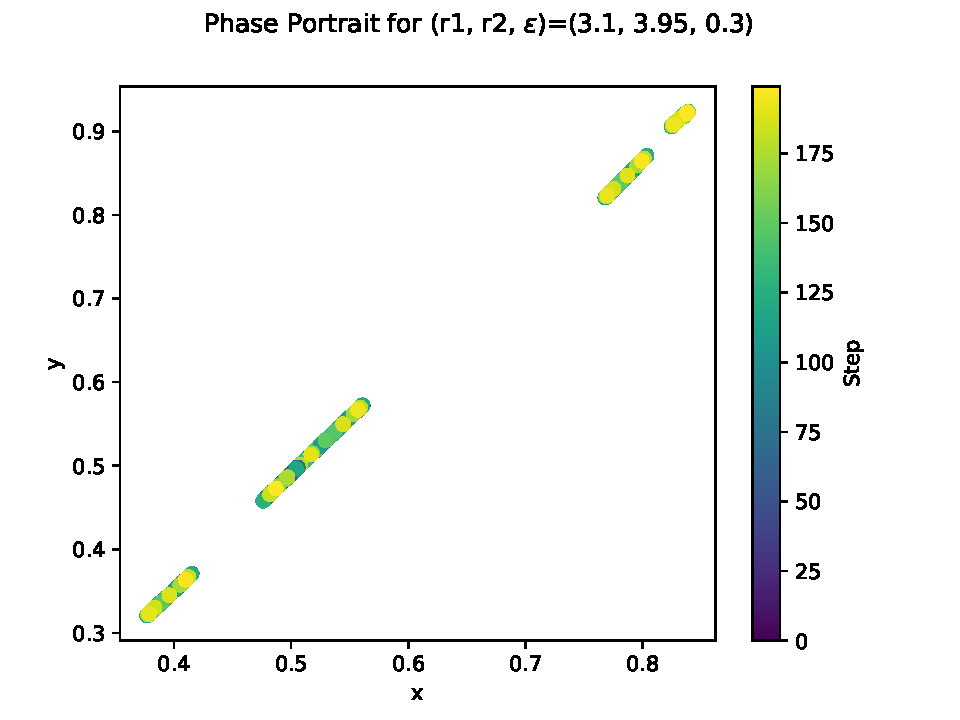
\includegraphics{figs/phase_(3.1, 3.95, 0.3)}
	\caption{Phase Portrait for $\left(r_1, r_2, \epsilon\right) = \left(3.1, 3.95, 0.2\right)$}
	\label{fig:phaseport-3.1-3.95}
\end{figure}
When further increasing $r_2$, this goes into the chaotic region of $r$ for the simple logistic map.
The impact on the coupled map we explore here can be seen in figure \ref{fig:phaseport-3.1-3.95}.
Here we can identify four distinct region in the phase portrait, all of which do not have a single point of convergence inside them but a certain spread and seem to be aligned along a common line.
The sizes of the regions vary significantly, the smallest is in the top right corner at around $(x, y) = (0.84, 0.92)$ and the largest region as at approximately $(x, y) = (0.53, 0.54)$ with a spread of around $0.5$ in both coordinates, slightly more so in the $y$-direction than the $x$-direction.
\newpage

\begin{figure}[h]
	\centering
	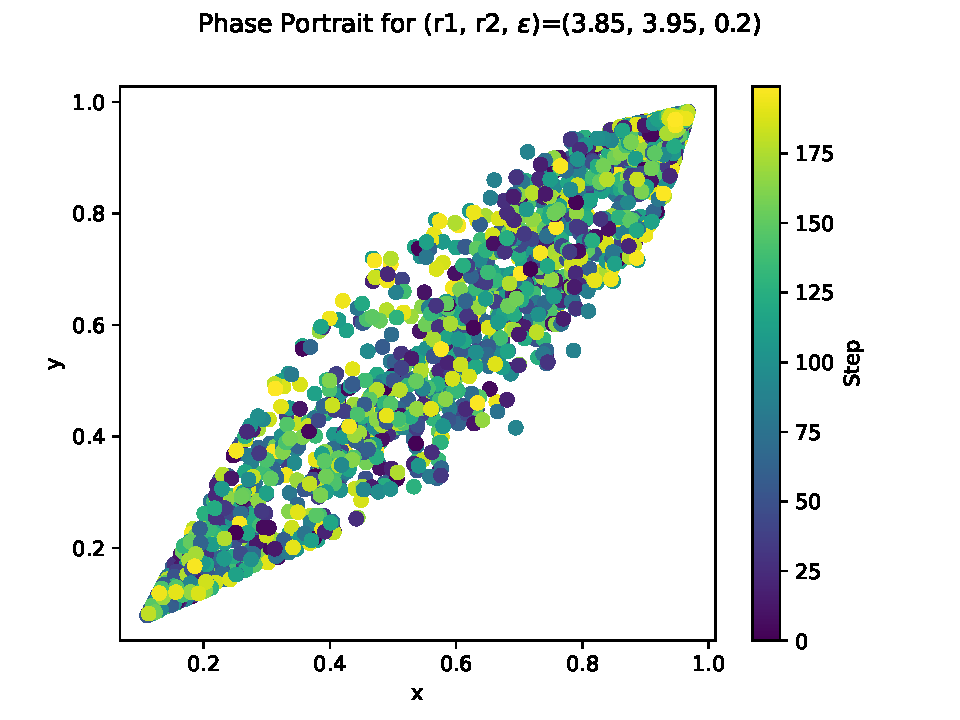
\includegraphics{figs/phase_(3.85, 3.95, 0.2)}
	\caption{Phase Portrait for $\left(r_1, r_2, \epsilon\right) = \left(3.85, 3.95, 0.2\right)$}
	\label{fig:phaseport-3.85}
\end{figure}
The best picture of obvious chaos is figure \ref{fig:phaseport-3.85}.
Here there is no discernible correlation in the distribution of points between the location in the plane and the temporal position in the evolution.
All the points together form a kind of almond shape which is wider in the centre and almost a point at both ends of the shape.
The shape is oriented almost along the diagonal but not quite because the scaling parameters $r_1$ and $r_2$ are once again chosen to be slightly different but are both in the chaotic regime.
\clearpage